\section{Come trovare $R$ nel caso generale}

\textbf{Come risolvere problemi di conduzione stazionaria}

\[
\begin{cases}
\mathrm{div}\,\vec{J} = 0 \\
\vec{E_c} \text{ conservativo } \Rightarrow \vec{E_c} = -\nabla V \\
\vec{E_c} = \rho \vec{J}, \quad \vec{J} = \gamma \vec{E_c}
\end{cases}
\]

\[
\mathrm{div}\,\vec{J} = \mathrm{div}(\gamma \vec{E_c}) 
   = -\,\mathrm{div}(\gamma \nabla V) = 0
\]

\[
\text{(Equazione di Laplace)}
\]

\[
\text{Se ho lo stesso materiale (omogeneo)} 
   \Rightarrow \gamma = \text{costante} 
   \Rightarrow \mathrm{div}(\nabla V) = \nabla^2 V = 0
\]

\[
\boxed{\nabla^2 V = 0}
\]
\begin{center}
    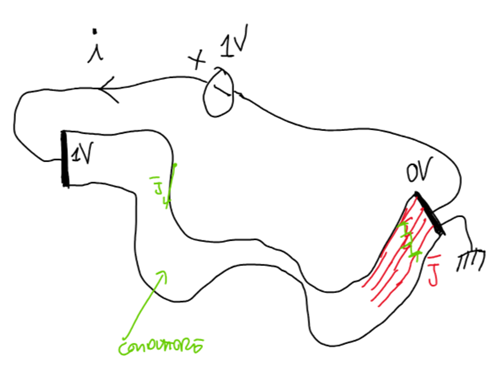
\includegraphics[scale = 0.5]{immagini/image16.png}
\end{center}
\subsection*{Bisogna specificare le condizioni al contorno}

\begin{enumerate}
    \item \textbf{Condizione di Dirichlet:} assegno il valore di $V$ su tutto il bordo.  
    \hfill (soluzione unica)
    
    \item \textbf{Condizione di Neumann:} assegno il valore di $\dfrac{\partial V}{\partial n}$ su tutto il bordo.  
    \hfill (infinite soluzioni in $V$ $\vec{E_c} = -\nabla V$)

    \item \textbf{Condizione “mista”} la soluzione è unica.
\end{enumerate}

\subsection*{Dal punto di vista fisico}
\begin{enumerate}[label=\alph*)]
  \item I morsetti sono \textbf{equipotenziali}.
  \item D.D.P. tra i morsetti è fissata (1V) $\Rightarrow \text{Applico condizioni di Dirichlet sui morsetti.}$
  \item  Sulla parte restadnte di bordo: $\vec{J} \cdot \hat{n} = J_n = 0$
\end{enumerate}

Le soluzioni del problema di Laplace sono dette \textbf{funzioni armoniche}.  
Il valore o i minimi di queste funzioni stanno su $\partial V$.

\[
\begin{cases}
\mathrm{div}\,\vec{E_c} = 0 \\[6pt]
\mathrm{rot}\,\vec{E_c} = 0
\end{cases}
\]

\[
\oint_{l_c} \vec{E_c} \cdot \hat{t}\, dl = 0 
\quad \Longleftrightarrow \quad 
\mathrm{rot}\,\vec{E_c} = 0
\]

\begin{center}
    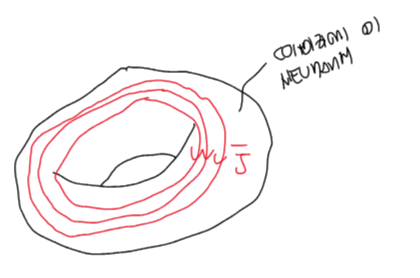
\includegraphics[scale = 0.7]{immagini/image17.png}
\end{center}

\section{Componente: Generatore elettrico}

È una porzione del tubo di flusso di $\vec{J}$, dove: $\vec{E_t} = \vec{E_c} + \vec{E_g}$

\begin{enumerate}
  \item $\vec{E_g}$ provoca una separazione di carica sui morsetti.
  \item Con la separazione di carica si genera un campo $\vec{E_c}$.
\end{enumerate}

\paragraph{Caso 1:} 
\textit{“A vuoto”} non connettiamo nulla al generatore che faccia scorrere una corrente.

\medskip
Quando si realizza l’equilibrio, le cariche restano ferme $\Rightarrow$ \textbf{elettrostatica.}

\[
\vec{E_t} = \rho \vec{J} = \rho \cdot 0 = 0 = \vec{E_c} + \vec{E_g}
\]

\[
\boxed{\vec{E_c} = -\vec{E_g}}
\]

se connettiamo il voltmetro ai capi del generatore:
\[
u_V = \int_{B,l_{EST}}^A \vec{E_t} \cdot \hat{t}\, dl 
    = \int_{B,l_{INT}}^A \vec{E_c} \cdot \hat{t}\, dl
    = \int_{B,l_{INT}}^A (-\vec{E_g}) \cdot \hat{t}\, dl 
    = \int_{A,l_{INT}}^B \vec{E_g} \cdot \hat{t}\, dl = e_{BA} = u_{BA}
\]
\noindent
\textit{(lettura del voltmetro)}  
\[
\text{Forza elettromotrice (FEM) del generatore:} \quad
e_{BA} = \int_A^B \vec{E_g} \cdot \hat{t}\, dl
\]
\[
\mu_{BA} = \int_B^A \vec{E_c} \cdot \hat{t}\, dl, 
\quad \text{e } \quad \mu_{BA} = e_{BA}
\]
\begin{center}
    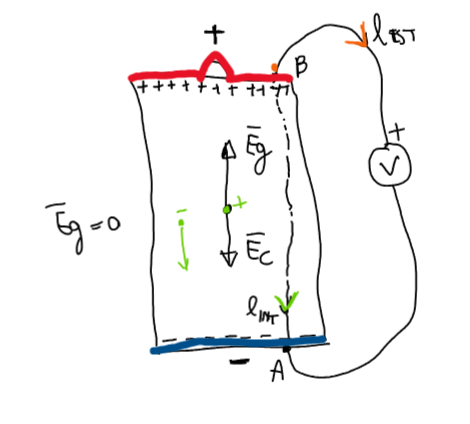
\includegraphics[scale = 0.7]{immagini/image18.png}
\end{center}

\subsection{Caso 2:}
“A carico” il generatore eroga una corrente $i$.

\[
\vec{E_t} = \rho \vec{J} = \vec{E_c} + \vec{E_g} \neq 0
\]

\[
R = \frac{1}{i} \int_A^B \vec{E_t} \cdot \hat{t}\, dl 
  = \frac{1}{i} \left( \int_A^B \vec{E_c} \cdot \hat{t}\, dl 
  + \int_A^B \vec{E_g} \cdot \hat{t}\, dl \right)
\]

\[
R = \frac{u_{AB} + e_{BA}}{i}
  = \frac{u_{BA} + e_{BA}}{i}
\]
\[
u_{BA} = e_{BA} - Ri
\]

\subsection{Bilancio di potenza nei generatori}
    \[
        Pe = u_{BA} \cdot i = (e_{BA} - Ri)\cdot i = e_{BA}i - Ri^2
    \]
    La potenza erogata è pari alla potenza generata meno la potenza dissipata per effetto Joule sulla R, nel caso di un GIT la dissipazione di potenza sulla resistenza è nulla (non c'è R).
\section{N-Poli}
    Gli N-Poli sono componenti con N morsetti, si può vedere come un tratto di tubo di flusso di $\vec{J}$ ramificato.
    \subsection{Proprietà}
        Siamo in \textbf{conduzione stazionaria} $\;\Rightarrow\; \mathrm{div}\,\vec{J}=0$ 

\[
\oint_{\partial V}\vec{J}\cdot\hat{n}\,dS=0
= \int_{S_L}\vec{J}\cdot\hat{n}\,dS
  + \sum_{j=1}^{N}\int_{S_j}\vec{J}\cdot\hat{n}_j\,dS
\]
\emph{$\vec{J}$ tangenziale su $S_L$. \;($S_j$ = superfici dei \textit{morsetti})}

\subsection*{3-polo (caso generale $N$)}
\[
\sum_{j=1}^{N} i_j = 0
\]
\emph{($i_j$ = corrente uscente dal morsetto $j$-esimo).}

\subsection*{Applicazione al bipolo: $N=2$}
\[
i_1 + i_2 = 0
\qquad\Longrightarrow\qquad
i_1 = -\,i_2
\]

\subsection*{Porta elettrica}
\textbf{Definizione:} una coppia di \textit{morsetti} in cui la corrente che entra da un morsetto esce dall’altro.

\subsection*{$M$-bipolo}
È un $N$-polo, con N = 2M, in cui i morsetti sono raggruppati in $M$ \textit{porte}.

\paragraph{Esempio}
$N=4,\; M=2 \;\Rightarrow\;$ \textit{4-polo}, \textit{2-porte}.

\subsection{Potenza elettrica scambiata da $N$-polo e $M$-bipolo}

Troviamo la potenza \textbf{uscente} da un $N$-polo:

\[
P_{\text{usc}} = - \int_{\tau} \vec{E_c} \cdot \vec{J}\, dv 
               = \oint_{\partial \tau} V \, \vec{J} \cdot \hat{n}\, dS
\]

\[
= \cancel{\int_{S_L} V\,\vec{J}\cdot\hat{n}_l\, dS}
  + \sum_{j=1}^{N} \int_{S_j} V\,\vec{J}\cdot\hat{n}_j\, dS
\]

Poiché $\vec{J}$ è tangente su $S_L$: $\Rightarrow \int_{S_L} V\,\vec{J}\cdot\hat{n}\, dS = 0$

Se $S_j$ è la superficie equipotenziale del morsetto $j$-esimo, $V = V_j$ costante su $S_j$:

\[
P_{\text{usc}} = \sum_{j=1}^{N} 
V_j \int_{S_j} \vec{J}\cdot\hat{n}_j\, dS
\]

Definendo:
\[
i_j = \int_{S_j} \vec{J}\cdot\hat{n}_j\, dS
\quad \text{(corrente del morsetto $j$-esimo)}
\]

\[
\boxed{
P_{\text{usc}} = \sum_{j=1}^{N} V_j\, i_j
}
\]


